\documentclass[11pt,a4paper,oneside]{article}

\usepackage{olymp}
%\usepackage{bnf}
\usepackage{amsfonts}
\usepackage{amsthm}
\usepackage{mathtools}
\usepackage{listings}
\usepackage{xcolor}
\usepackage{etoolbox}
\usepackage{graphicx}
\usepackage{wrapfig}
\usepackage{afterpage}
\usepackage{float}
\usepackage{pgffor}
\usepackage{fancyvrb}
\usepackage{tikz}
\usepackage{caption}

\usepackage[ruled, vlined]{algorithm2e}
\usepackage[spanish]{babel}
\usepackage[utf8]{inputenc}

\newtheorem*{proposition*}{Proposición}

\definecolor{codegray}{rgb}{0.5,0.5,0.5}
\definecolor{codepurple}{rgb}{0.58,0,0.82}
\definecolor{backcolour}{rgb}{0.95,0.95,0.92}

% Code style definition
\lstdefinestyle{codeStyle}{
  backgroundcolor=\color{backcolour},
  commentstyle=\color{codepurple}\ttfamily,
  morecomment=[l][\color{magenta}]{\#},
  keywordstyle=\color{blue}\ttfamily,
  numberstyle=\tiny\color{codegray},
  stringstyle=\color{red}\ttfamily,
  basicstyle=\ttfamily,
  breakatwhitespace=false,         
  breaklines=true,                 
  captionpos=b,                    
  keepspaces=true,                 
  numbers=left,                    
  numbersep=5pt,                  
  showspaces=false,                
  showstringspaces=false,
  showtabs=false,                  
  tabsize=2
}
\lstset{style=codeStyle}

% Balloon
\newcommand{\balloon}[1]{
   \begin{minipage}{0cm}{
        \vspace*{-0.5cm}
        \hspace*{3.0cm}
        \smash{
            \begin{tikzpicture}[overlay, scale=.25]
                \definecolor{ballooncolor}{HTML}{#1}
                \definecolor{fakewhite}{HTML}{ffffcc}
                \tikzstyle{balloon}=[outer color=ballooncolor,inner color=ballooncolor!30!fakewhite];
                \shade[ball color=ballooncolor] (-.1,-2) -- (-.3,-2.2) -- (.3,-2.2) -- (.1,-2) -- cycle;
                \draw (0,-2.2) .. controls (-0.5,-2.8) and (-0.5,-3.4) .. (0,-4);
                \draw (0,-4) .. controls (0.5,-4.6) and (0.5,-5.2) .. (0,-5.8);
                \draw[thick] ellipse (1.75 and 2);
                \clip ellipse (1.75 and 2);
                \shade[balloon] (-.5,.5) circle (3);
            \end{tikzpicture}
        }
    }
   \end{minipage}
}

% Vars definition for document test
%\def\cuscontestName{CUSCONTEST TEST}
%\def\cuscontestDate{Cusco, 14 de Julio de 2024}
%\def\folderpath{template}
%\def\folderlist{CombinacionDeLaCerradura}

% Vars definition for document
\def\cuscontestName{CUSCONTEST XXI}
\def\cuscontestDate{Cusco, 02 de Agosto de 2024}
\def\cuscontestProblemset{Este problemset contiene 13 problemas etiquetados de la `A' a la `M'.}
\def\description{description.tex}
\def\editorial{editorial.tex}
\def\folderpath{2024}
% ADD HERE YOUR FOLDER PROBLEM USING COMMA SEPARATOR
\def\folderlist{
Zanahorias,
DecodificacionMaya,
NumeroDeSerie,
Empacando,
Nohana,
BrigadaAntiTerrorista-I,
BrigadaAntiTerrorista-II,
RedDeTransporte,
MejorTrayecto,
irishpub,
ChifaInusual-I,
ChifaInusual-II,
Civilizaciones}

% New commands
\renewcommand{\contestname}{
    \cuscontestName \\
    \cuscontestDate
}

\newcommand{\problemText}[6]{
    \begin{problem}{#1}{#2}{#3}{#4}{#5}{#6}
}

\newcommand{\inputText}{
    \InputFile
}

\newcommand{\outputText}{
    \OutputFile
}

\newcommand{\exampleCases}{
    \Example
}

\newcommand{\caseFile}[1]{
    \VerbatimInput{#1}
}

\newcommand{\explanationText}{
    \Explanation
}

\newcommand{\editorialText}[1]{
    \vspace*{0cm}
    {\Large\textbf{Solución:}}\\
    \textbf{Conocimientos requeridos:} #1.\\
}

\newcommand{\code}[2]{
    \vspace{0.7cm}
    \textbf{Implementación en #1:}
    \vspace{0.25cm}
    \lstinputlisting[language=#1,style=codeStyle]{#2}
}

% Main document
\begin{document}
    % Provide problems and editorial
    \providetoggle{solution}
    \settoggle{solution}{true}
    %\settoggle{solution}{false}

    % Layer page
    \clearpage\thispagestyle{empty}

\begin{figure}
    \centering
    \begin{minipage}{.32\textwidth}
        \centering
        
\includegraphics[height=.40\linewidth]{images/logo_cp.png}
    \end{minipage}
    \begin{minipage}{.32\textwidth}
        \centering
        
\includegraphics[height=.53\linewidth]{images/logo_acm.png}
    \end{minipage}
    \begin{minipage}{.32\textwidth}
        \centering
        
\includegraphics[height=.22\linewidth]{images/logo_omegaup.png}
    \end{minipage}
\end{figure}

\begin{center}
    \large
    UNIVERSIDAD NACIONAL DE SAN ANTONIO ABAD DEL CUSCO\\
    \vspace{0.3cm}
    FACULTAD DE INGENIERÍA ELÉCTRICA, ELECTRÓNICA, INFORMÁTICA Y MECÁNICA\\
    \vspace{0.3cm}
    ESCUELA PROFESIONAL DE INGENIERÍA INFORMÁTICA Y DE SISTEMAS\\
    \vspace{2cm}
    ACM CHAPTER CUSCO\\
    \vspace{2cm}
    \Large
    CONCURSO DE PROGRAMACIÓN\\
    \vspace{0.5cm}
    \Huge{\textbf{\cuscontestName}}\\
    \Large
    \vspace{0.5cm}
    \iftoggle{solution}{\textit{PROBLEMSET CON SOLUCIONES}}{\textit{PROBLEMSET}}
    \\
    \vspace{3cm}
    \large
    \cuscontestDate\\
    \vspace{3cm}
    \cuscontestProblemset
\end{center}

    \newpage
    
    % Informations page
    \clearpage\thispagestyle{empty}

{\Large \textbf{Información General}}\\
A menos que se indique lo contrario, las siguientes condiciones son válidas para todos los problemas.\\

\textbf{Nombre del programa}
\begin{enumerate}
    \item La solución debe ser enviada en formatos del lenguaje seleccionado. Ejemplo: codigo.c, codigo.cpp, codigo.java, codigo.py, codigo.cs.
\end{enumerate}

\textbf{Entrada}
\begin{enumerate}
    \item La entrada debe ser leída desde la entrada estándar (consola).
    \item La entrada consiste en un único caso de prueba, que es descrito en el formato de cada problema. No existen datos extras en la entrada.
    \item Cuando una línea de datos contiene muchos valores, estos son separados por exactamente un espacio entre ellos. No existen otros espacios en las entradas.
    \item Se utiliza el alfabeto inglés. No hay letras con tildes, diéresis, eñes, u otros símbolos.
\end{enumerate}

\textbf{Salida}
\begin{enumerate}
    \item La salida debe ser escrita como salida estándar (consola).
    \item El resultado debe ser escrito en la cantidad de líneas especificada para cada problema. No debe imprimirse otros datos. Ejemplo: no incluir: ``ingrese el número''.
    \item Cuando una línea de datos de salida contiene muchos valores, estos deben ser separados por exactamente un espacio entre ellos. No deben imprimirse otros espacios en las salidas.
    \item Debe ser utilizado el alfabeto Inglés. No letras con tildes, diéresis, eñes, u otros símbolos.
\end{enumerate}

\textbf{Límite de Tiempo}
\begin{enumerate}
    \item El límite de tiempo informado para cada problema corresponde con el tiempo total permitido para la ejecución completa de los casos de prueba.
\end{enumerate}

\textbf{Consejos}
\begin{enumerate}
    \item Para leer múltiples números en una línea en Python usa: A = [int(x) for x in input().split(' ')]
    \item Para soluciones en java, enviar el archivo .java sin el ``package name''.
    \item Para compilar con c++ y si el archivo se llama code.cpp usar el comando g++ code.cpp -o code y para ejecutar usar el comando ./code
\end{enumerate}

\begin{center}
    %\vspace{1cm}
    Problemas coordinados por Justino Ferro Alvarez, y planteados por:
    \vspace{0.2cm}
    \begin{tabular}{ l l l}
        \multicolumn{1}{c}{\textbf{Autor}} & \multicolumn{1}{c}{\textbf{Cargo}} & \multicolumn{1}{c}{\textbf{Institución}}  \\
        Berthin S. Torres Callanaupa & Software Engineer & Marvell Semicondutor, NL\\
        Dennis Huillca & Software Engineer & Tranzact, PE\\
        Edú Sanchez & Senior Software Engineer & Google, BR\\
        Grover Castro & PhD in Computer Sc. & Universität Leipzig, DE\\
        Isaac Campos & Team Lead &  Finbe USA\\
        Jared León & PhD Stud. in Maths & University of Warwick, UK\\
        Jhamsid Romero Bernal & Student & UNSAAC, PE\\
        Josué Nina & Data integration and ETL developer & Provista, USA\\
        Kleiber Ttito & Software Engineer & Amazon, USA \\        
    \end{tabular}
\end{center}

    \newpage

    % Problems and editorials
    \foreach \folder in \folderlist {
        \problemText{Dios Si Castiga Dos Veces}{Entrada estándar}{Salida estándar}{1 segundo}{}{Josue Nina}

Mi amigo Yerim es un gran fanático de la cultura Japonesa, ha invertido años en ello y ya cumple con las característica mas importante para ser considerado un otaku: No bañarse por mas de 3 días.

El gran sueño de Yerim es ser parte de un Isekai (un subgénero japonés que involucra personajes transportados a otro mundo, típicamente de fantasía o aventura), el invirtió años construyendo una maquina que permita lograr eso.
Finalmente llego el día en el que pondría a prueba su experimento, pero la maquina falló y como consecuencia lo llevo al pasado, específicamente a la China comunista de 1963.
Ahora Yerim es forzado a trabajar con una remuneración mínima haciendo letreros para el estado, dichos letreros solo pueden ser de dos tipos:
\begin{itemize}
	\item ACM (Asociación de Campesinos Maoístas)
	\item ICPC (Ilustre Colegio de Profesores Comunistas)
\end{itemize}

Yerim recibe una gran cantidad de letras mayúsculas y percibe un beneficio de 5 yuans por cada letrero que forme la palabra: "ACM" o "ICPC".

Cada letra solo puede ser usado en único letrero.


Determinar el máximo beneficio que puede obtener Yerim.

\inputText

En la primera línea tendrá un entero $t$ $(1 \leq t \leq10^3)$ indicando el número de casos de prueba, las siguientes $t$ líneas tendrá una cadena $s$ ($1\leq |s|\leq200$) que solo contiene letras mayúsculas del alfabeto.

\outputText

Para cada caso, imprimir el mayor beneficio que puede obtener Yerim.\\

\exampleCases

\begin{example}
    \exmp{%%INPUT
        \caseFile{2023/M_DiosSiCastigaDosVeces/in/1.in}
    }{%%OUTPUT
        \caseFile{2023/M_DiosSiCastigaDosVeces/out/1.out}
    }%%END-OUTPUT
\end{example}

\explanationText

\begin{figure}[H]
\centering
  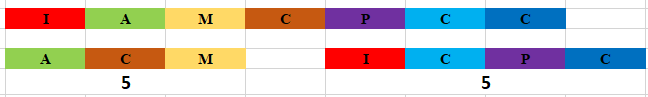
\includegraphics[width=15cm]{2023/M_DiosSiCastigaDosVeces/images/Screenshot_4.png}
\end{figure}
        \iftoggle{solution}{\newpage\editorialText{Teoría de grafos básica y combinatoria}

Dado que Lucho siempre puede comunicarse con todas las otras personas, es fácil ver
que se tiene un grafo conexo. Por lo que cada par de vértices puede conectarse entre
sí. Existen~${n \choose 2} = n(n - 1) / 2$ pares de vértices, siendo ésta la
respuesta siempre.

\code{C++}{2023/E_Sendero/solution.cpp}
}{}
        \newpage
    }
\end{document}
